\documentclass[a4paper,12pt]{article}
\usepackage[utf8]{inputenc}
\usepackage[spanish]{babel}
\usepackage{amsmath, amssymb}
\usepackage{graphicx}
\usepackage{geometry}
\usepackage{hyperref}
\usepackage{float}
\usepackage{fancyhdr}
\usepackage{tocloft}
\usepackage{caption}
\captionsetup[figure]{skip=2pt}
\geometry{margin=2.5cm}

% Encabezado y pie de página
\pagestyle{fancy}
\fancyhf{}
\lhead{Inferencia y Estimación}
\rhead{Universidad de San Andrés}
\cfoot{\thepage}


% Portada formal
\begin{document}
\noindent
\begin{minipage}{\textwidth}
    \centering
    {\scshape\LARGE Universidad de San Andrés \par}
    \vspace{1.2cm}
    {\scshape\Large Inferencia y Estimación\par}
    \vspace{1.2cm}
    {\huge\bfseries Compresión y Descompresión de Imágenes usando PCA\par}
    \vspace{1.5cm}
    {\large
    Catalina Hirsch - 36557 \\ Clara Zavaroni Benoit - 36772 \\ Maylen Antonella Villagrán Cardozo - 36758 \\}
    \vspace{1cm}
    {\large \today\par}
\end{minipage}



\begin{abstract}
La realización de este trabajo práctico tiene como objetivo aplicar el método de \textbf{Análisis de Componentes Principales (PCA)} en la compresión de imágenes. Se busca reducir el espacio de almacenamiento minimizando la pérdida de información, conservando los datos que contienen la mayor parte de la varianza. Posteriormente, se descomprime la imagen y se compara con la original para evaluar la calidad de la compresión, utilizando métricas objetivas. El desempeño se evalúa en función de la cantidad de componentes principales utilizados. Finalmente, se discuten los resultados y conclusiones obtenidas.
\end{abstract}


\section*{Introducción}
\addcontentsline{toc}{section}{Introducción}
En este informe se estudia la compresión y descompresión de imágenes mediante el método de Análisis de Componentes Principales (PCA). Se analizan las propiedades estadísticas de las imágenes, se implementa el proceso de compresión y reconstrucción, y se evalúa el desempeño en función de la calidad de la imagen reconstruida y el ahorro de espacio.
\newpage
\section*{Ejercicio 1: Correlación}
\addcontentsline{toc}{section}{Ejercicio 1: Correlación}
El propósito de este ejercicio es analizar el comportamiento de los píxeles vecinos en las imágenes utilizadas. En primer lugar, se cargan las imágenes y se convierten a escala de grises. Luego, se divide cada imagen en bloques de 2x1 píxeles contiguos verticalmente. A continuación, se calcula la correlación entre los píxeles de cada bloque y se almacena en un vector. Finalmente, se realiza un gráfico de dispersión de las correlaciones obtenidas para cada imagen. Los resultados se presentan a continuación:

\begin{figure}[H]
    \centering
    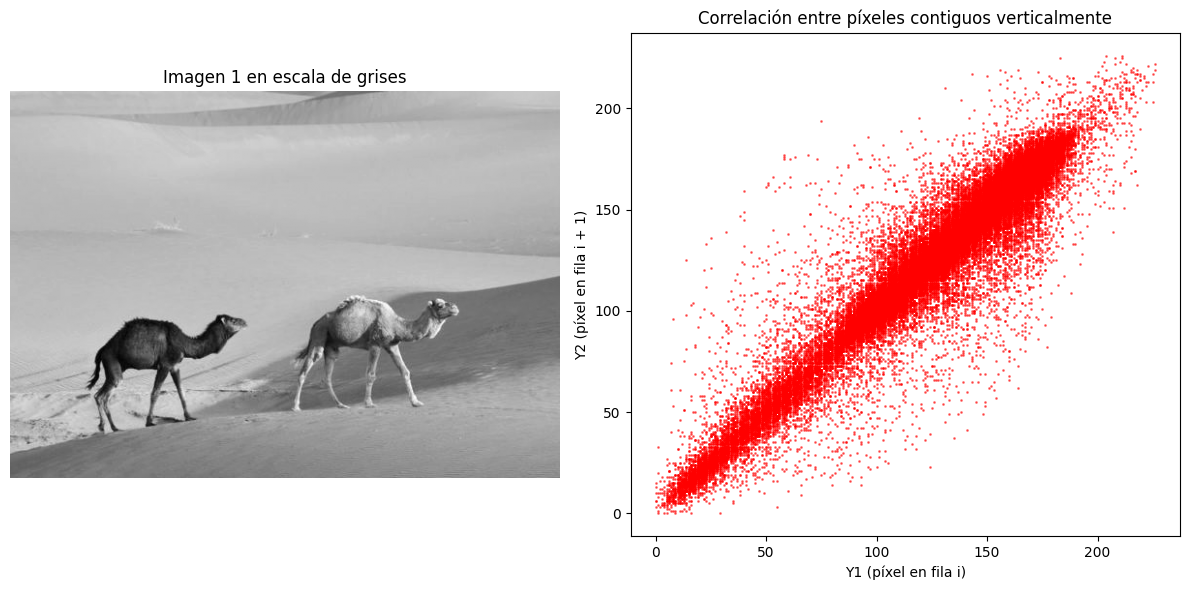
\includegraphics[width=1\textwidth]{Ejercicio1a.png}
    \caption{Imagen 1, gráfico de dispersión de la correlación de píxeles contiguos verticalmente}
    \captionsetup{belowskip=0pt}
    \label{fig:correlacion1}
\end{figure}
\vspace{-1em}
Analizando el comportamiento del gráfico, los puntos se alinean en torno a una recta creciente, lo cual indica una fuerte correlación positiva entre los píxeles.
El resultado se debe a que, la imagen presenta suavidad, el color de los píxeles vecinos se asemeja.
Por otro lado, los resultados de la segunda imagen son los siguientes:
\vspace{-1em}
\begin{figure}[H]
    \centering
    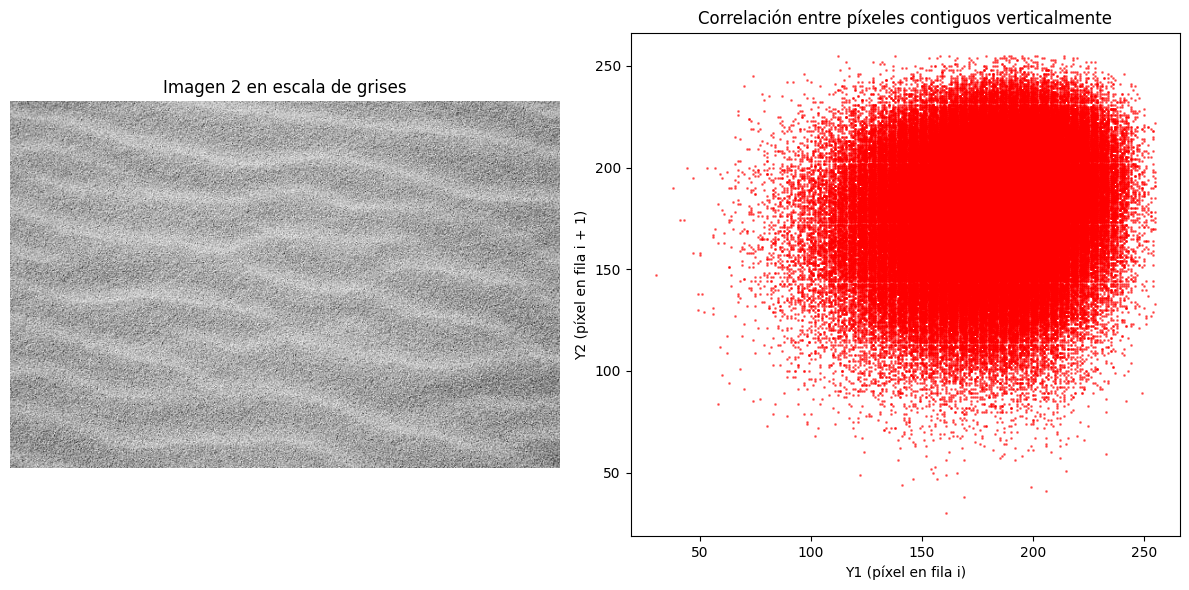
\includegraphics[width=1\textwidth]{Ejercicio1b.png}
    \caption{Imagen 2, gráfico de dispersión de la correlación de píxeles contiguos verticalmente}
    \captionsetup{belowskip=0pt}
    \label{fig:correlacion2}
\end{figure}
A diferencia del gráfico anterior, los puntos se encuentran más dispersos, implicando una correlación más baja que la imagen anterior.
Atribuimos la diferencia al ruido perteneciente a esta imagen, y a la falta de suavidad. Los colores entre los píxeles vecinos no están relacionados.

Luego, se estimó el coeficiente de correlación de cada vector. Los resultados son los presentados a continuación:
\begin{enumerate}
    \item Para la Imagen 1 se obtuvo: 
    Coeficiente de correlación: 0.9789354535355658

    \item Para la Imagen 2 se obtuvo: 
    Coeficiente de correlación: 0.1460473239944978
\end{enumerate}

Los resultados de la primera imagen apoyan lo intuido anteriormente, al aproximarse al valor 1, indican una fuerte correlación entre los píxeles.
Con respecto a la segunda imagen, sus resultados también apoyan lo intuido, al acercarse al valor 0.1, demuestra que los píxeles vecinos no están relacionados.

\vspace{1em}

La diferencia entre ambas imágenes nos indica cuál se podría comprimir con mayor calidad. En primer lugar, la imagen 1 al comprimirse, podría eliminar la redundancia entre píxeles vecinos.
Evitando perder la calidad de la imagen. En cambio, en la imagen 2, la falta de redundancia causa la pérdida de calidad al momento de comprimir, ya que se dificulta la predicción de un píxel a partir de su vecino. 

\vspace{1em}

Por último, se pide una transformación que descorrelacione las variables.
Se utiliza la transformación de descorrelación de PCA:

\vspace{1em}

\[
Y = P^T X
\]
De esta forma, \(Y\) es la proyección de \(X\) en el espacio de autovectores de \(C_X\).

Nuevamente, se hace uso de un gráfico de dispersión por imagen, dando los siguientes resultados:

\begin{figure}[H]
    \centering
    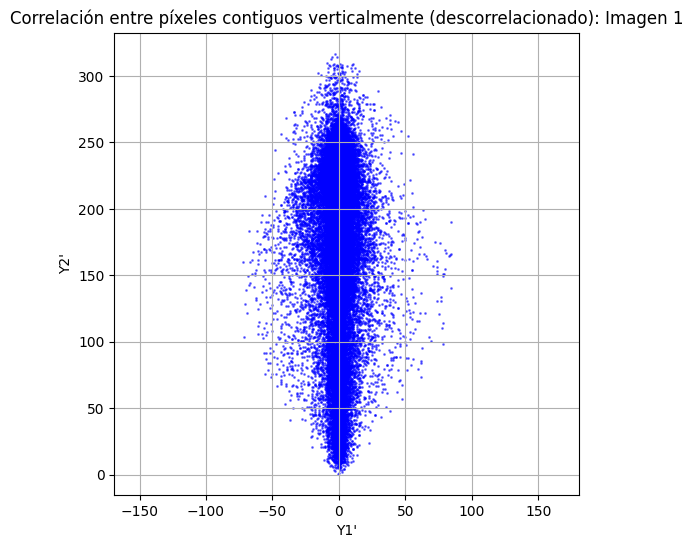
\includegraphics[width=0.6\textwidth]{Ejercicio1c.png}
    \caption{Imagen 1, gráfico de dispersión de la descorrelación de píxeles contiguos verticalmente}
    \label{fig:descorrelacion1}
\end{figure}
\vspace{-1em}
Podemos observar en la primera imagen cómo los píxeles se encuentran concentrados en el eje vertical Y2, el proceso de descorrelación resulta exitoso.
\vspace{-1em}
\begin{figure}[H]
    \centering
    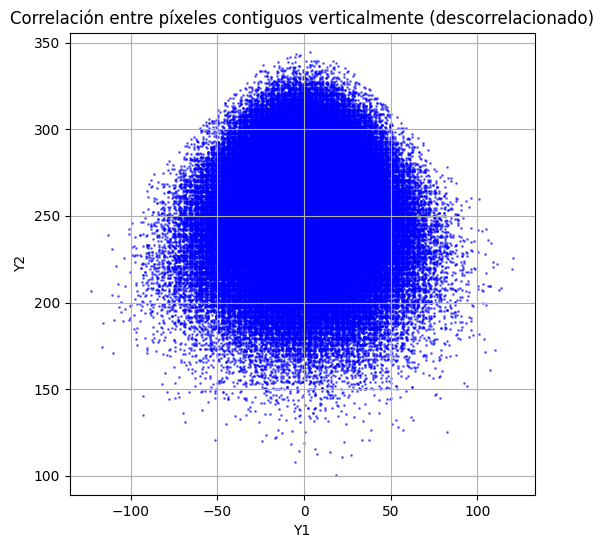
\includegraphics[width=0.6\textwidth]{Ejercicio1d.png}
    \caption{Imagen 2, gráfico de dispersión de la descorrelación de píxeles contiguos verticalmente}
    \label{fig:descorrelacion2}
\end{figure}

Por otro lado, en la segunda imagen, el gráfico se mantiene en forma de una nube, como en la Figura 2, demostrando la falta de correlación inicial.
\newpage
\section*{Ejercicio 2: Compresión}
\addcontentsline{toc}{section}{Ejercicio 2: Compresión}

En este ejercicio se implementa un método de compresión de imágenes utilizando el Análisis de Componentes Principales (PCA). El objetivo es transformar la información contenida en la imagen, originalmente de alta dimensión, en una representación más compacta que conserve la mayor parte de la información relevante.

\vspace{1em}

El proceso comienza dividiendo la imagen en bloques de 8x8 píxeles. Cada uno de estos bloques se recorre por columnas y se convierte en un vector columna de 64 elementos. De esta manera, si la imagen tiene un total de $m$ bloques, se obtiene una colección de vectores $\mathbf{x}_1, \mathbf{x}_2, \ldots, \mathbf{x}_m$, cada uno de dimensión $64 \times 1$. Estos vectores se organizan como filas en una matriz de datos $X$ de tamaño $m \times 64$, donde cada fila representa un bloque vectorizado y cada columna corresponde a una posición fija dentro del bloque.

\vspace{1em}

Para analizar la estructura estadística de los datos, primero se calcula el vector media $\boldsymbol{\mu}$, que contiene el promedio de cada columna de $X$. Matemáticamente, esto se expresa como:
\[
\boldsymbol{\mu} = \frac{1}{m} \sum_{i=1}^m \mathbf{x}_i
\]
Luego, se centra la matriz de datos restando la media a cada fila, obteniendo así la matriz centrada $X_c = X - \mathbf{1}_m \boldsymbol{\mu}^T$, donde $\mathbf{1}_m$ es un vector columna de unos de dimensión $m$.

\vspace{1em}

El siguiente paso consiste en calcular la matriz de covarianza $C_X$, que describe cómo varían conjuntamente las distintas posiciones dentro de los bloques. Esta matriz se estima mediante:
\[
C_X = \frac{1}{m-1} X_c^T X_c
\]
Cada elemento $c_{ij}$ de $C_X$ representa la covarianza entre la posición $i$ y la posición $j$ dentro de los bloques.

\vspace{1em}

Para aplicar PCA, se resuelve el problema de autovalores y autovectores de la matriz de covarianza. Es decir, se buscan vectores $\mathbf{v}_j$ y escalares $\lambda_j$ que satisfagan:
\[
C_X \mathbf{v}_j = \lambda_j \mathbf{v}_j
\]
Los autovalores $\lambda_j$ se ordenan de mayor a menor, y se seleccionan los $k$ más grandes, que corresponden a las direcciones de mayor varianza en los datos. Los autovectores asociados se agrupan en la matriz de proyección $P$:
\[
P = [\mathbf{v}_1, \mathbf{v}_2, \ldots, \mathbf{v}_k]
\]
La proyección de los datos originales sobre este subespacio de menor dimensión se obtiene multiplicando la matriz centrada $X_c$ por $P$, resultando en la matriz $Y$ de datos comprimidos:
\[
Y = X_c P
\]
El número de componentes $k$ a conservar se determina en función del factor de compresión deseado. En el código, la función \texttt{space\_saving\_k(s, m)} calcula $k$ como:
\[
k = \max\big(1, \min(m, \lceil m(1-s) \rceil)\big)
\]
donde $s$ es el porcentaje de reducción elegido, con valores entre 0 y 1.

\vspace{1em}

Finalmente, para permitir la reconstrucción de la imagen comprimida, se almacenan la matriz $Y$ de datos comprimidos, la matriz de autovectores $P$ y el vector de medias $\boldsymbol{\mu}$. La reconstrucción aproximada de la imagen original se realiza aplicando la transformación inversa:
\[
\hat{X} = Y P^T + \mathbf{1}_m \boldsymbol{\mu}^T
\]
Además, se grafica el espectro de autovalores $\lambda_j$ para visualizar cuánta información se conserva y cuánta se descarta al reducir la dimensionalidad.

\newpage
\section*{Ejercicio 3: Descompresión}
\addcontentsline{toc}{section}{Ejercicio 3: Descompresión}

Luego de lo realizado en el Ejercicio 2, se realiza la reconstrucción de la imagen comprimida utilizando el proceso inverso del PCA de compresión, para descomprimir.
A través del Ejercicio 2, se obtienen los siguientes datos de la imagen:

\vspace{1em}

Vectores \(y_i\) (\(Y\)), la matriz de autovectores (\(P\)) y la media \(\mu_X\) (\(\mu\))

\vspace{1em}

Una vez obtenida la información indicada, se aplica la proyección inversa del PCA, para obtener los vectores \(x_i\) aproximados:

\vspace{1em}

\[
X = Y P^T + \mu
\]
donde \(X\) es la matriz original, \(Y\) es la matriz proyectada, \(P\) son los autovectores y \(\mu\) es la media.

\vspace{1em}

Finalmente, se recorre una matriz vacía, del tamaño necesario de la imagen, completando con los bloques de la imagen reconstruida.
De esta manera, obtenemos los siguientes resultados:

\begin{figure}[H]
    \centering
    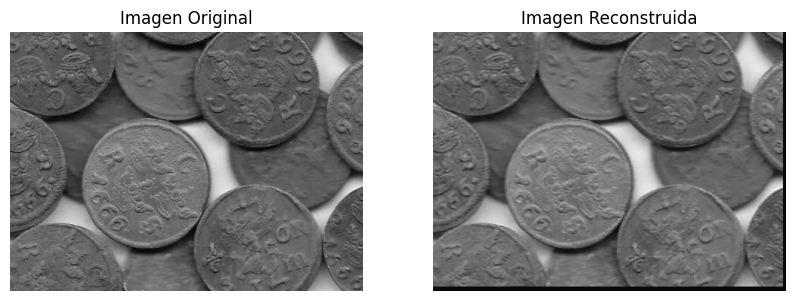
\includegraphics[width=1\textwidth]{Ejercicio3.png}
    \caption{Imagen reconstruida a través del proceso de PCA inverso.}
    \label{fig:ej3}
\end{figure}

Podemos notar el borde negro de la imagen reconstruida, lo cual sucede al no poder completar bloques de exactamente 8 * 8 al comprimir la imagen.
Adicionalmente, podemos observar una diferencia entre las imágenes o pérdida de nitidez, atribuida a la reducción de la dimensionalidad y la eliminación de componentes de menor varianza.

\newpage
\section*{Ejercicio 4: Medidas de desempeño}
\addcontentsline{toc}{section}{Ejercicio 4: Medidas de desempeño}
El objetivo de este ejercicio es evaluar el desempeño de la compresión de imágenes al variar el espacio ahorrado (S). 

\begin{equation}
S = \left( 1 - \frac{\text{cantidad de componentes principales } (k)}{\text{cantidad de componentes totales } (m)} \right) \times 100 \%
\end{equation}

En primer lugar, para cada porcentaje de espacio ahorrado comprimimos una imagen y la reconstruimos. Luego, para 
medir el rendimiento del procedimiento, calculamos el error cuadrático medio (MSE) entre la imagen original y 
la reconstruida. 
\begin{equation}
MSE = \frac{1}{N_w N_h} \sum_{i=1}^{N_w} \sum_{j=1}^{N_h} (p_{ij} - \hat{p}_{ij})^2
\end{equation}

\begin{figure}[H]
    \centering
    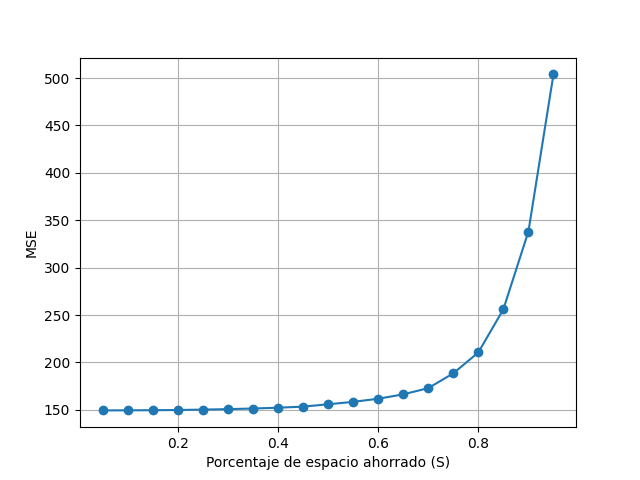
\includegraphics[width=1\textwidth]{Ejercicio 4a.png}
    \caption{Gráfico MSE vs S}
    \label{fig:ej4}
\end{figure}

En el gráfico, se observa que el error cuadrático medio aumenta a medida que lo hace el espacio ahorrado.
Este resultado es coherente, ya que al descartar un mayor número de componentes principales se pierde más 
información de la imagen. 
Sin embargo, esta relación no es proporcional: el error crece considerablemente a partir de un espacio 
ahorrado del 80\%. Al superar ese porcentaje, la pérdida de información se vuelve significativa, 
impactando notablemente en la calidad de la imagen. 


Para ilustrarlo, incluimos algunas imágenes para diferentes porcentajes de espacio ahorrado. 
\begin{figure}[H]
    \centering
    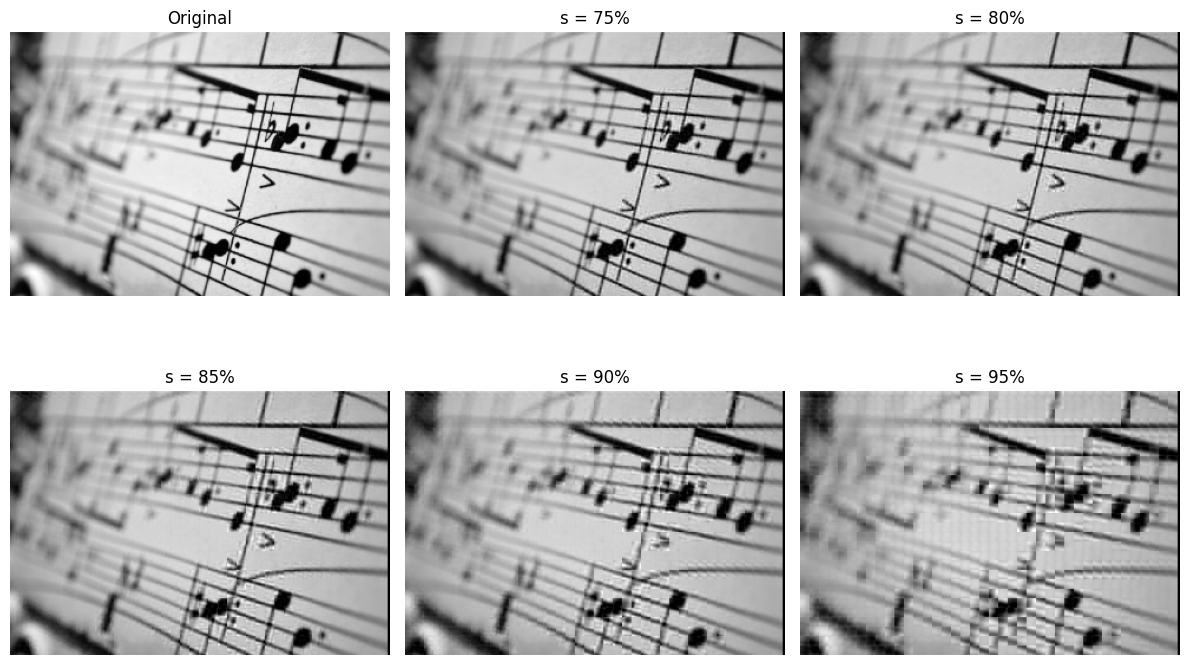
\includegraphics[width=1\textwidth]{Ejercicio 4b.png}
    \caption{Imagen original vs las reconstruidas para diferentes S.}
    \label{fig:ej4b}
\end{figure}

Vemos que a medida que S aumenta, la imagen reconstruida pierde nitidez. La reducción de 
componentes principales se ve en una disminución de la calidad de la imagen. 

\newpage
\section*{Conclusiones}
\addcontentsline{toc}{section}{Conclusiones}
En este trabajo práctico implementamos y evaluamos la compresión de imágenes usando 
PCA (Análisis de Componentes Principales). Este permite reducir la dimensión de los datos
al descartar las componentes de menor varianza, quedándose con las componentes principales, 
es decir aquellas necesarias para la comprensión de la imagen. De esta manera, se ahorra espacio 
sin comprometer significativamente la calidad de la imagen.

\vspace{1em}

Los resultados mostraron que, a medida que aumenta el porcentaje de espacio ahorrado, la calidad
de la imagen reconstruida decae progresivamente, especialmente a partir de la reducción de 80\%. 
Esto se refleja en un incremento notable del MSE. Sin embargo, consideramos que
para valores intermedios de compresión (cercanos al 70\%), obtenemos un buen balance entre nitidez 
de la imagen y reducción de memoria. 

\vspace{1em}

*problemas??*

\vspace{1em}

En conclusión, la aplicación de PCA para la compresión de imágenes nos permitió observar
de primera mano cómo la reducción de dimensionalidad ayuda en el ahorro de almacenamiento,
sin comprometer demasiado la calidad de la imagen.

\end{document}
